\documentclass[12pt, spanish]{article}
\usepackage[spanish]{babel}
\selectlanguage{spanish}
%\usepackage{natbib}
\usepackage{url}
\usepackage[utf8x]{inputenc}
\usepackage{graphicx}
\graphicspath{{images/}}
\usepackage{parskip}
\usepackage{fancyhdr}
\usepackage{vmargin}
\usepackage{multirow}
\usepackage{float}
\usepackage{chngpage}

\usepackage{amsfonts}

\usepackage{subcaption}

\usepackage{hyperref}
\usepackage[
    type={CC},
    modifier={by-nc-sa},
    version={4.0},
]{doclicense}

\hypersetup{
    colorlinks=true,
    linkcolor=blue,
    filecolor=magenta,      
    urlcolor=cyan,
}

% para codigo
\usepackage{listings}
\usepackage{xcolor}



%% configuración de listings

\definecolor{listing-background}{HTML}{F7F7F7}
\definecolor{listing-rule}{HTML}{B3B2B3}
\definecolor{listing-numbers}{HTML}{B3B2B3}
\definecolor{listing-text-color}{HTML}{000000}
\definecolor{listing-keyword}{HTML}{435489}
\definecolor{listing-identifier}{HTML}{435489}
\definecolor{listing-string}{HTML}{00999A}
\definecolor{listing-comment}{HTML}{8E8E8E}
\definecolor{listing-javadoc-comment}{HTML}{006CA9}

\lstdefinestyle{eisvogel_listing_style}{
  language         = python,
%$if(listings-disable-line-numbers)$
%  xleftmargin      = 0.6em,
%  framexleftmargin = 0.4em,
%$else$
  numbers          = left,
  xleftmargin      = 0em,
 framexleftmargin = 0em,
%$endif$
  backgroundcolor  = \color{listing-background},
  basicstyle       = \color{listing-text-color}\small\ttfamily{}\linespread{1.15}, % print whole listing small
  breaklines       = true,
  frame            = single,
  framesep         = 0.19em,
  rulecolor        = \color{listing-rule},
  frameround       = ffff,
  tabsize          = 4,
  numberstyle      = \color{listing-numbers},
  aboveskip        = 1.0em,
  belowskip        = 0.1em,
  abovecaptionskip = 0em,
  belowcaptionskip = 1.0em,
  keywordstyle     = \color{listing-keyword}\bfseries,
  classoffset      = 0,
  sensitive        = true,
  identifierstyle  = \color{listing-identifier},
  commentstyle     = \color{listing-comment},
  morecomment      = [s][\color{listing-javadoc-comment}]{/**}{*/},
  stringstyle      = \color{listing-string},
  showstringspaces = false,
  escapeinside     = {/*@}{@*/}, % Allow LaTeX inside these special comments
  literate         =
  {á}{{\'a}}1 {é}{{\'e}}1 {í}{{\'i}}1 {ó}{{\'o}}1 {ú}{{\'u}}1
  {Á}{{\'A}}1 {É}{{\'E}}1 {Í}{{\'I}}1 {Ó}{{\'O}}1 {Ú}{{\'U}}1
  {à}{{\`a}}1 {è}{{\'e}}1 {ì}{{\`i}}1 {ò}{{\`o}}1 {ù}{{\`u}}1
  {À}{{\`A}}1 {È}{{\'E}}1 {Ì}{{\`I}}1 {Ò}{{\`O}}1 {Ù}{{\`U}}1
  {ä}{{\"a}}1 {ë}{{\"e}}1 {ï}{{\"i}}1 {ö}{{\"o}}1 {ü}{{\"u}}1
  {Ä}{{\"A}}1 {Ë}{{\"E}}1 {Ï}{{\"I}}1 {Ö}{{\"O}}1 {Ü}{{\"U}}1
  {â}{{\^a}}1 {ê}{{\^e}}1 {î}{{\^i}}1 {ô}{{\^o}}1 {û}{{\^u}}1
  {Â}{{\^A}}1 {Ê}{{\^E}}1 {Î}{{\^I}}1 {Ô}{{\^O}}1 {Û}{{\^U}}1
  {œ}{{\oe}}1 {Œ}{{\OE}}1 {æ}{{\ae}}1 {Æ}{{\AE}}1 {ß}{{\ss}}1
  {ç}{{\c c}}1 {Ç}{{\c C}}1 {ø}{{\o}}1 {å}{{\r a}}1 {Å}{{\r A}}1
  {€}{{\EUR}}1 {£}{{\pounds}}1 {«}{{\guillemotleft}}1
  {»}{{\guillemotright}}1 {ñ}{{\~n}}1 {Ñ}{{\~N}}1 {¿}{{?`}}1
  {…}{{\ldots}}1 {≥}{{>=}}1 {≤}{{<=}}1 {„}{{\glqq}}1 {“}{{\grqq}}1
  {”}{{''}}1
}
\lstset{style=eisvogel_listing_style}


\usepackage[default]{sourcesanspro}

\setmarginsrb{2 cm}{1 cm}{2 cm}{2 cm}{1 cm}{1.5 cm}{1 cm}{1.5 cm}

\title{Práctica 3:\\
Programación  \hspace{0.05cm} }                           
\author{Antonio David Villegas Yeguas}                             
\date{\today}                                           

\renewcommand*\contentsname{hola}

\makeatletter
\let\thetitle\@title
\let\theauthor\@author
\let\thedate\@date
\makeatother

\pagestyle{fancy}
\fancyhf{}
\rhead{\theauthor}
\lhead{\thetitle}
\cfoot{\thepage}

\begin{document}

%%%%%%%%%%%%%%%%%%%%%%%%%%%%%%%%%%%%%%%%%%%%%%%%%%%%%%%%%%%%%%%%%%%%%%%%%%%%%%%%%%%%%%%%%

\begin{titlepage}
    \centering
    \vspace*{0.3 cm}
    
\includegraphics[scale = 0.50]{ugr.png}\\[0.7 cm]
    %\textsc{\LARGE Universidad de Granada}\\[2.0 cm]   
    \textsc{\large 3º CSI 2019/20 - Grupo 1}\\[0.5 cm]            
    \textsc{\large Grado en Ingeniería Informática}\\[0.5 cm]              
    \rule{\linewidth}{0.2 mm} \\[0.2 cm]
    { \huge \bfseries \thetitle}\\
    \rule{\linewidth}{0.2 mm} \\[1 cm]
    
    \begin{minipage}{0.4\textwidth}
        \begin{flushleft} \large
            \emph{Autor:}\\
            \theauthor\\ 
			 \emph{DNI:}\\
            77021623-M
            \end{flushleft}
            \end{minipage}~
            \begin{minipage}{0.4\textwidth}
            \begin{flushright} \large
            \emph{Asignatura: \\
            AA}   \\     
            \emph{Correo:}\\
            advy99@correo.ugr.es           
        \end{flushright}
    \end{minipage}\\[0.5cm]
  
    {\large \thedate}\\[0.5cm]
    %{\url{https://github.com/advy99/AA/}}
    {\doclicenseThis}
 	
    \vfill
    
\end{titlepage}

%%%%%%%%%%%%%%%%%%%%%%%%%%%%%%%%%%%%%%%%%%%%%%%%%%%%%%%%%%%%%%%%%%%%%%%%%%%%%%%%%%%%%%%%%

\tableofcontents
\pagebreak

%%%%%%%%%%%%%%%%%%%%%%%%%%%%%%%%%%%%%%%%%%%%%%%%%%%%%%%%%%%%%%%%%%%%%%%%%%%%%%%%%%%%%%%%%


\section*{Introducción}

Para esta práctica se pide explicar el proceso a realizar para resolver dos problemas de aprendizaje utilizando los modelos lineales vistos a lo largo de la teoría y prácticas de la asignatura.

Para esta práctica utilizaré la biblioteca Scikit-Learn\cite{sklearn} ya que cuenta con todas las herramientas que utilizaré y explicaré más adelante. No usé esta herramienta en prácticas anteriores ya que se nos pedía implementar los algoritmos y herramientas, sin embargo para esta práctica nos será más sencillo utilizarla.

\section{Problema de clasificación.}

\subsection{Comprender el problema. Identificar X, Y y F en el problema.}

En este problema tenemos datos sobre imágenes de números escritos a mano por un total de 43 personas, los números escritos por 30 de estas son el conjunto de training dado y los números de las 13 personas restantes conforman el conjunto de test. Estos datos se han obtenido de la base de datos \textit{Machine Learning Repository}, en concreto usaremos el conjunto de datos \textit{Optical Recognition of Handwritter Digits Data Set} \cite{mlr_digitos}.

Cada número se representa como una imagen de 32 por 32 bitmaps, donde 1 representa que en dicha posición se ha escrito y un 0 no. Como podemos leer en la descripción del \textit{data set}, los datos que usamos están preprocesados, en lugar de tener una matriz 32 por 32 se han separado en bloques de 4 por 4 sin solapamiento de forma que tenemos una matriz 8 por 8, 64 valores entre 0 a 16,0 si el bloque no tiene ningún pixel en negro y 16 si todos los píxeles del bloque son negros.

Los ficheros de datos de entrada cuentan con 65 columnas por cada fila, los 64 valores de la imagen y por último la clase a la que pertenece dicho dato. Explicaré que significa cada valor y que clases posibles pueden tomar en las siguientes secciones.

\subsubsection{X del problema.}

El conjunto X del problema son los datos de entrada con los que entrenaremos el modelo. 

Como leemos del fichero de información de descripción disponible en la base de datos\cite{mlr_digitos}, cada dato x cuenta con 64 variables cuyo valor está en el rango [0,16], cada variable representa una sección 4 por 4 de la imagen leída del número, si el valor es 16 quiere decir que la sección está por completo escrita, y un 0 que ninguno de sus píxeles está escrito el valor.

Comprobaremos que esto efectivamente es así cuando hablemos sobre los conjuntos de training y test más adelante.

\subsubsection{Y del problema.}

Las etiquetas del problema representan los valores escritos en la entrada, es decir, un dato leído tendrá sus 64 valores correspondientes a la información de la imagen leída y la etiqueta será un valor entre [0,9] que representa el valor escrito en la imagen.

\subsubsection{F del problema.}

La función $f$ del problema es la función desconocida que clasifica de forma perfecta cualquier número. El objetivo de esta práctica es obtener una función $g$ perteneciente al conjunto de clases de funciones a usar (del que hablaré más adelante) que sea lo más parecida posible a la función $f$.

Este problema lo podemos tratar como un problema de aprendizaje ya que los datos cuentan con un patrón (si a una entrada le damos una etiqueta es muy probable que las entradas similares tengan la misma etiqueta), la función $f$ es desconocida y no es calculable, ya que si lo fuera no necesitamos utilizar técnicas de aprendizaje, simplemente aplicamos la función y hemos resuelto el problema, y por último, tenemos datos con los que entrenar nuestro modelo.

\subsection{Clases de funciones a usar.}

Para este problema utilizaré combinaciones lineales de los datos. Dado que las características de los datos de entrada son la cantidad de unos que hay en una zona de la matriz que representa la imagen no tiene sentido aplicar transformaciones no lineales a los valores, es decir, no tiene ningún significado aplicar el cuadrado a un número de bits.

Otra razón es que el problema ya es de gran dimensionalidad, si usamos clases de funciones más complejas podría presentar problemas de overfitting o una necesidad mayor de tiempo de entrenamiento.

\subsection{Conjuntos de training y test.}

El problema ya nos proporciona un conjunto de training y test separado, luego no tendremos que separarlos para este problema.

\subsubsection{Conjunto de training}

Tras leer los ficheros dados de training podemos comprobar los datos del problema. En este caso el conjunto dado de training cuenta con 3823 datos y como vimos en la introducción del problema, podemos comprobar que efectivamente cada dato tiene 64 variables:

\begin{figure}[H]
	\centering
	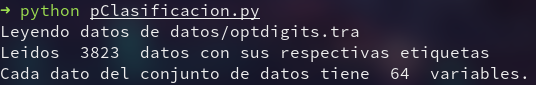
\includegraphics[scale=0.7]{clasificacion/num_datos.png}
	\caption{Información sobre el número de datos en training.}
	\label{datosClasificacion}
\end{figure}

De la lectura de este fichero también podemos ver el reparto de los datos según su clase al estar realizando técnicas de aprendizaje supervisado (como hemos hecho en anteriores prácticas y también haremos en esta):

\begin{figure}[H]
	\centering
	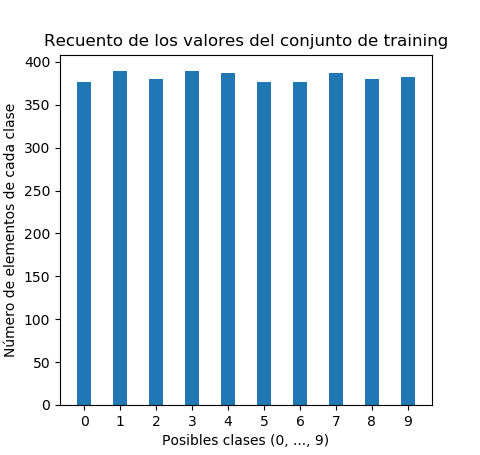
\includegraphics[scale=1]{clasificacion/datos_tra.png}
	\caption{Información sobre la clase de los datos en training.}
	\label{claseDatosClasificacion}
\end{figure}

Como podemos ver el número de elementos de cada clase está equilibrado, luego en principio no debería generar problemas al entrenar nuestro modelo. Es importante que en el conjunto de training se de este equilibrio y se encuentren datos de todas las clases, ya que en caso contrario podría ocurrir que en el conjunto de test o incluso fuera de la muestra fallemos al intentar clasificar un dato que contiene información sobre una clase desconocida al entrenar, pero como podemos ver, este no es el caso.

\subsubsection{Conjunto de validación}

A partir del conjunto de entrenamiento obtendré un conjunto para realizar la validación del modelo. Usaré cross-validation a través de las herramientas que ofrece Scitik-Learn para realizar la validación cruzada\cite{crossval}, aunque comentaré en la sección de hiperparámetros el número de particiones de validación. 

Este método consiste en dividir los datos de entrenamiento, de forma que tengamos un conjunto de entrenamiento más pequeño y $k$ conjuntos de validación ($k$ es un entero que discutiré en la sección de hiperparámetros), de forma que se entrenará $k$  veces y se validará con las $k$ particiones de validación, y finalmente nos quedaremos con la media de estas, para asegurar tener un buen ajuste.

\subsubsection{Conjunto de test}

En el fichero que nos proporcionan con los datos de test vemos que tenemos 1797 datos (bastantes menos que en el conjunto de training), pero como es de esperar, cada dato usa la misma representación, es decir, está compuesto por 64 características y la clase a la que pertenece:

\begin{figure}[H]
	\centering
	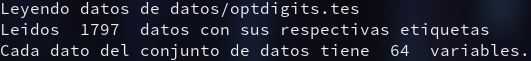
\includegraphics[scale=0.7]{clasificacion/num_datos_test.png}
	\caption{Información sobre el número de datos  en test.}
	\label{datosClasificacionTest}
\end{figure}


Con respecto al número de datos por clase, en este conjunto también vemos que tenemos una distribución uniforme de los datos entre las clases, aunque en este caso no es importante al no usar este conjunto para el entrenamiento, es decir, este conjunto de datos solo lo usaremos para comprobar como se comportan los distintos modelos.

\begin{figure}[H]
	\centering
	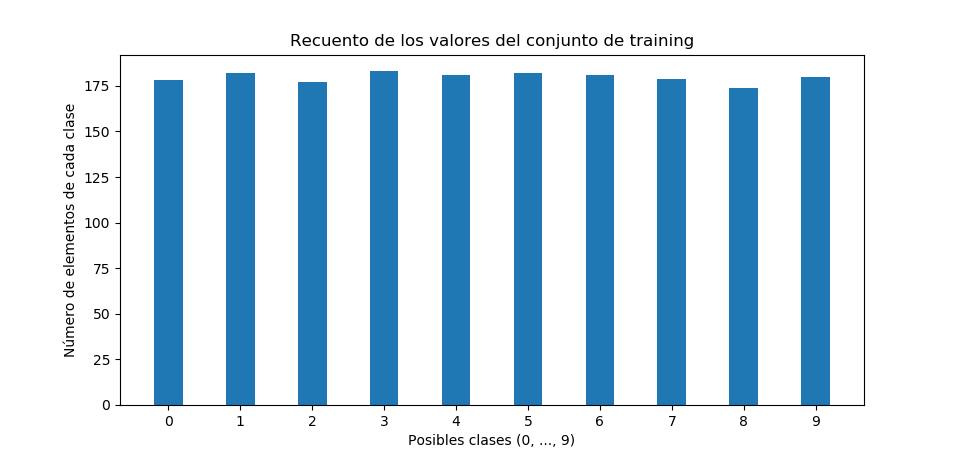
\includegraphics[scale=0.7]{clasificacion/datos_test.png}
	\caption{Información sobre la clase de los datos en test.}
	\label{claseDatosTestClasificacion}
\end{figure}

\newpage

\subsection{Preprocesado de los datos.}

Como he comentado con respecto a los datos de este problema, en el repositorio de donde se han extraído los datos nos avisan de que estos ya se encuentran preprocesados, inicialmente los datos eran un bitmap con valores 0 o 1 representado en una matriz de 32 por 32, que se ha preprocesado de forma que se ha dividido en secciones de bitmap 4 por 4 sin solapamiento, es decir, los datos ya preprocesados son una matriz con valores entre 0 y 16 en la que cada posición representa un cuadrante 4 por 4, de ahí que el valor esté entre 0 (el bitmap de la sección no tenia ningún valor como 1) a 16 (todos los valores del bitmap en esa sección 4 por 4 valen 1).

Los valores todos están en un rango fijo que es el mismo para todos (entre 0 y 16), por lo que en principio no va a afectar, por lo que no lo modificaré. Es posible que en esta sección aparezca una nota en la que si finalmente se ha obtenido mejor resultado normalizando los valores entre 0 y 1 se ha aplicado esa transformación a los datos (básicamente consiste en dividir todos los datos por 16 para que se encuentren en el rango [0, 1]).

\subsection{Fijar la métrica. Idoneidad sobre el problema.}

\subsection{Técnica de ajuste elegida.}

\subsection{Necesidad de regulación.}

\subsection{Modelos a usar.}


\subsubsection{Regresión Lineal.}

\subsubsection{Regresión Lineal con regularización (Ridge Regression).}


\subsubsection{Gradiente Descendente Estocástico.}


\subsection{Hiperparámetros y selección del mejor modelo.}

\subsection{Estimación del error fuera de la muestra usando validación cruzada y comparación con el error en test.}

\subsection{Modelo propuesto y estimación del error fuera de la muestra de este modelo.}




\newpage

\section{Problema de regresión.}

\subsection{Comprender el problema. Identificar X, Y y F en el problema.}


\subsubsection{X del problema.}


\subsubsection{Y del problema.}

\subsubsection{F del problema.}

\subsection{Clases de funciones a usar.}

\subsection{Conjuntos de training y test.}

\subsection{Preprocesado de los datos.}

\subsection{Fijar la métrica. Idoneidad sobre el problema.}

\subsection{Técnica de ajuste elegida.}

\subsection{Necesidad de regulación.}

\subsection{Modelos a usar.}

\subsection{Hiperparámetros y selección del mejor modelo.}

\subsection{Estimación del error fuera de la muestra usando validación cruzada y comparación con el error en test.}

\subsection{Modelo propuesto y estimación del error fuera de la muestra de este modelo.}


\newpage


\section{Referencias, material y documentación usada}


\begin{thebibliography}{9}


\bibitem{sklearn}
Página web de Scikit Learn
\url{https://scikit-learn.org/stable/user_guide.html}


\bibitem{mlr_digitos}
Machine Learning Repository: Optical Recognition of Handwritten Digits Data Set 

\url{https://archive.ics.uci.edu/ml/datasets/optical+recognition+of+handwritten+digits}


\bibitem{crossval}
\url{https://scikit-learn.org/stable/modules/generated/sklearn.model_selection.cross_val_score.html}



\bibitem{ridge}
\url{https://scikit-learn.org/stable/modules/generated/sklearn.linear_model.Ridge.html#sklearn.linear_model.Ridge}

\bibitem{sgdclasificacion}
\url{https://scikit-learn.org/stable/modules/generated/sklearn.linear_model.SGDClassifier.html#sklearn.linear_model.SGDClassifier}

\bibitem{mlr_crimen}
Machine Learning Repository: Communities and Crime Data Set  

\url{http://archive.ics.uci.edu/ml/datasets/Communities+and+Crime}

\bibitem{sklearn-linearmodel}
\url{https://scikit-learn.org/stable/modules/linear_model.html}

\bibitem{sklearn-model-selection}
\url{https://scikit-learn.org/stable/modules/classes.html#module-sklearn.model_selection}

\end{thebibliography}

\end{document}
